\section{Filtering 3D Shared Surrounding Environments}
\label{sec:surrounding:environment}

In this work \cite{Nassani2018b}, we explore the social sharing of surrounding environments on wearable AR devices. In particular, we propose filtering the level of detail of sharing the surrounding environment based on the social proximity between the viewer and the sharer. We test the effect of having the filter (varying the levels of detail) on the shared surrounding environment, to preserve the sense of privacy from both viewer and sharer perspectives, and conducted a study using the HoloLens. We report on semi-structured questionnaire results and suggest future directions in the social sharing of surrounding environments.

This work explores new ways of sharing the remote environment of social contacts in a wearable AR interface. We build on top of our previous work \cite{Nassani2018a} that looked into sharing surrounding environments based on social proximity. Previously, we tested three levels of representing surrounding environments: 360-degree video, 2d Video and 2D Image. This work focuses on sharing 3D captured rooms and levels of detail that can be used based on social proximity. The significance of the work is that it addresses the privacy concerns of the sharer as well as the efficiency of placing the surrounding AR space of the viewer.

\subsection{Prototype}

When the user puts on the HoloLens, he/she sees an AR user interface (UI) showing simulated social contacts (see Figure~\ref{fig:environment:setup}). The UI displays the social contacts around the viewer. Above each social contact avatar, the viewer can see a representation of the shared remote surrounding environment. The level of detail of the shared surrounding environment is determined by the social proximity to the viewer.

The user can air-tap on the environment above an avatar to expand it to life-size around the avatar (Figure~\ref{fig:environment:environment-levels}). The user can walk inside and explore the shared surrounding environment.

\begin{figure*}
    \centering
    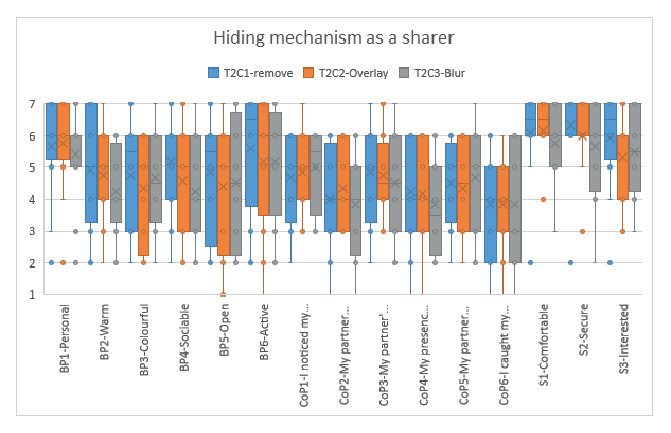
\includegraphics[width=\columnwidth]{images/ismar18/images-06.eps}
    \caption{The viewer uses the HoloLens to view social contacts and proximity-filtered shared environments.}
    \label{fig:environment:setup}
\end{figure*}

\begin{figure}[ht]
  \centering
  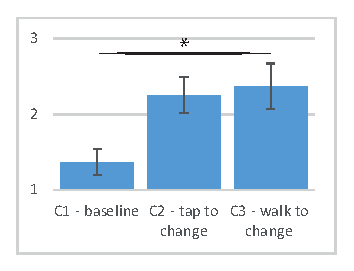
\includegraphics[width=2in]{images/ismar18/images-05.eps}
  \caption{Levels of detail of the shared surrounding environment. 1) full details for Intimate contact: including family picture, bank balance and computer monitor. 2) partial details for Friend contact: hiding the family picture, bank balance, but keeping work-related items such as computer monitor. 3) limited details for Stranger contact: hidden personal and work related items.}
  \label{fig:environment:environment-levels}
\end{figure}

\begin{figure}[t]
  \centering
  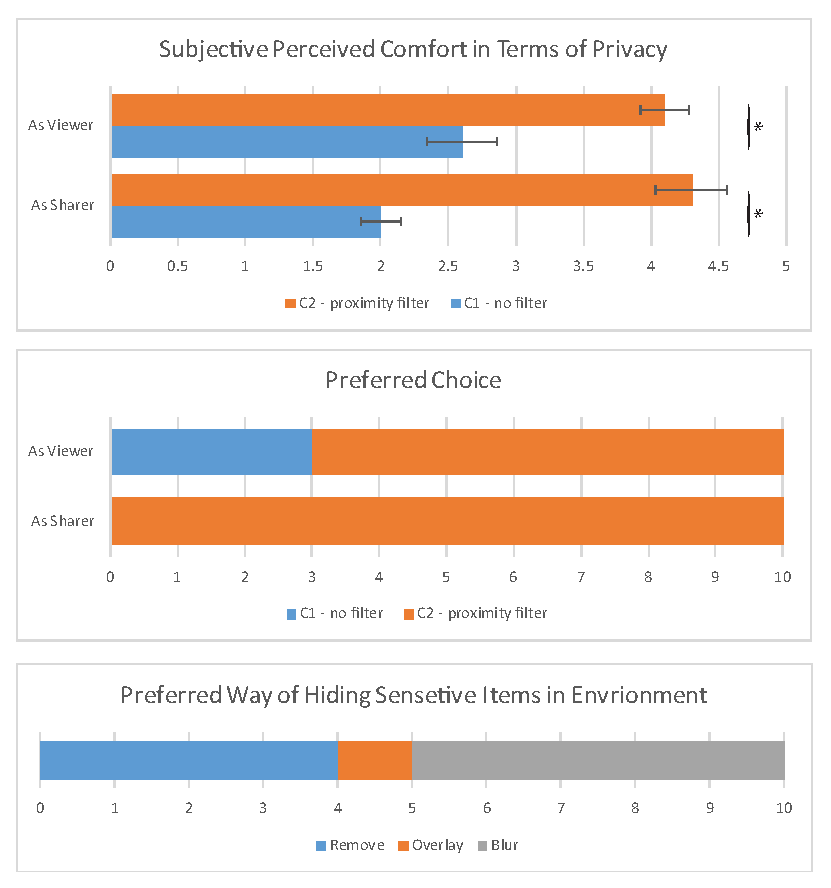
\includegraphics[width=\columnwidth]{images/ismar18/images-04.eps}
  \caption{Top: the average results of subjective comfort questions. Middle: the percentage results of ranking the best condition. Bottom: the percentage results of voting for the best method to hide part of the environment. Whiskers indicate the standard error.}
  \label{fig:environment:results}
\end{figure}


The prototype was built using the Microsoft HoloLens\footnote{https://www.microsoft.com/en-us/hololens} and the Mixed Reality Toolkit\footnote{https://github.com/Microsoft/MixedRealityToolkit-Unity}. The avatars representing the social contacts were generated using MakeHuman\footnote{http://www.makehumancommunity.org/}. The 3D representation of the remote sharer's room was modelled in AutoDesk Maya\footnote{https://www.autodesk.com/products/maya/overview} to simulate 3D scanning of the user's surrounding environment. To test if users preferred to have a proximity filter applied on the shared surrounding environment, the prototype offers to turn the filter on or off in two conditions; a base-line (C1: no-filter) and a proximity filter applied (C2: proximity-filter).


\subsection{User Study}

We collected feedback from 10 participants (five female) with an average age of 28.8 ($SD=3.65$). The participants tried demonstrations of the two conditions: C1 (no filter), where all social contacts are sharing the full view of their surrounding environments, and C2 (proximity filter), where the shared surrounding environments are filtered based on three levels of social proximity (Intimate, Friend and Stranger) mapped to the level of detail of the shared surrounding environment (Full, Partial and Limited). The order of the conditions was randomised based on a Latin square. 

For each condition, we asked participants to rate how comfortable they felt (on a five-point Likert scale) about the sharing environment from the perspective of a sharer (person sharing) and the viewer (the person viewing) of the surrounding environment. We also asked participants to rank which condition they preferred (and to state why) from both perspectives. Finally, we asked about which method of hiding sensitive items in the shared environment the user preferred by selecting an option from 1) remove/hide the item as if it did not exist, 2) block/overlay a black box on the item so it will be hidden, 3) blur out the item, 4) other. 

We ran a Wilcoxon signed-rank test on the subjective perceived comfort in terms of privacy. The test showed that having a proximity filter (C2) applied on the shared surrounding environment did elicit a statistically significant improvement in perceived comfort in terms of privacy for both sharers ($Z=-2.831$, $p=0.005$) and viewers ($Z=-2.588$, $p=0.01$). 

As for the ranking results, C2 (proximity filter) was preferred by both sharers (100\%) and viewers (70\%) over C1 (no filter). C1 (no filter) was ranked 30\% for viewers. In terms of the preferred way of hiding sensitive items in the shared environment, blurring sensitive items (60\%) was preferred followed by removing/hiding sensitive items as if they did not exist (40\%) and the lowest was overlay (10\%). 

In the open-ended questions, C1 (no filter) was reported stronger in terms of the curiosity for the viewer. "... would suit supervisors who are interested in knowing details about their social network", one participant mentioned. The most reported strength of C2 (proximity filter) was around privacy and the sense of being comfortable in sharing levels based on social proximity. 

Overall, the results confirm our hypothesis of the value of social proximity-based filtering for sharing the surrounding environment. An interesting observation is that the sharer perspective may be different from the viewer perspective in terms of privacy. In the future, we will extend this work to explore live (synchronous) sharing with both avatars and real people. Also, we will look into the perspective of sharer and how they can select which part of the room to share with which level of social proximity contact.

\subsection{Summary}

In this work, we explored implementing the social AR continuum on the shared surround spaces between social contacts. We ran a study to test the effect of applying a filter on levels of detail on how comfortable the participants were in terms of privacy. We found that most participants are more comfortable when the social filter was applied to the shared surrounding environment. 